\documentclass[twocolumn,a4,notitlepage]{article}

\usepackage[dvips]{graphicx}
%\usepackage{listings}
%\usepackage{url}
\usepackage{subfigure}

\include{epsf}

\title{Modelling Hole Transport in Slithering-Snake Simulated Blends of
Conjugated Polymers}
\author{Jenny Nelson, Jarvist Frost}
\begin{document}

\maketitle

\twocolumn[
\begin{abstract}
Blends of conjugated polymers were simulated by using a slithering-snake
Monte-Carlo algorithm. 
Two distinct 
three-dimensional structures arose, depending whether 
the polymers were homophilic or heterophilic. 
Time of
flight simulations were carried out with no energetic disorder, in order to
try and isolate the effect of morphology.

Homophilic polymers formed clumps, and it was demonstrated that a
quasi-equilibirium existed between local clumping and full phase separation,
which we believe is most indicative of experimental samples. The size of
clumps in this quasi-equilibrium was found to be highly temperature
dependent. Time of flight simulations produced dispersive transients with
positive mobility dependency on field.

Heterophilic polymers demonstrated a stable `lacework' pattern for densities
of above $16\%$. These structures offered enormous interfacial area between
the two polymers, and very low diffusion distances for an exciton to travel
before reaching a boundary. Time of Flight simulations indicated non-dispersive
(charge-sheet like) behaviour at low bias, which then became more 
dispersive as the bias increased.
This was understood in terms of the high bias causing `fish trap' structures
to appear where the carriers were trapped in `downstream' but non connecting
regions.

\bigskip
\end{abstract}
]

\section{Introduction}



\section{Morphology Generation}

Morphologies were generated by use of a Slithering-Snake monte carlo method.
A population of conjugated polymer chains (snakes) were drawn from a
Gaussian distribution of chain length with associated parameters $\bar{l}$ \&
$\sigma_l$, and then laid down randomly in the 3D lattice.

These polymer chains were constricted to move linearly, with one of the
heads extending itself by one unit in any of the three cartessian
directions. They were considered to be in a `sea' of other material, which
was displaced around the snake without energy cost.

For each `slither' of the monte-carlo simulation, a particular snake, head
and direction were chosen at random. A calculation was made of the energy
change associated with such a move, which came about as a result of the
interaction energies between lattice units of `snake' [conjugated polymer
oligomers] versus the `sea' of other plastic or the snake material itself. 

Due to the constrictions placed on the snake movement, and once
consideration was made for the energy associated with a configuration where
a certain snake touched itself, this calculation could be simplified to a
energy summation over the lattice site that the `head' was about to move
into, and the site that the `tail' was about to depart from. This
calculation is independent of chain length.

When this energy, $dE$, was negative then the exothermic movement progressed
automatically. For $dE>0$, the endothermic movement progressed if there was
sufficient Boltzman energy to drive it.

\section{Morphology Results}

Two fundamentally different morphologies were generated by setting the
Snake-Snake interaction energy either positive or negative, generating
homophilic and heterophilic polymer chains respectively. 
Due to the THATOTHERDUDESNAME
principle, a homophobic blend is equivalent to a heterophilic one - where
the polymers would energetically prefer to be in touch with each other.
A homophilic blend would be expected to phase phase separate, whereas a
heterophilic blend would prefer to be in a stable blend.

The percolation threshold of the two different blends was examined [Fig.
\ref{percolate}], and was found to be different for the two morphologies.
Homophilic blends went through a percolation boundary at between $20-30\%$,
whereas heterophilic blends began percolating at between $16-25\%$. 

\begin{figure}[htb]
\centering
\label{percolate}
\includegraphics[width=5cm,angle=270]{figures/percolate.eps}
\caption{Figure displaying the fraction of segments connected to the base
electrode by a percolating cluster, versus the density of the mix, for 
25-long chain pure blends of both homophilic \& heterophilic polymers.}
\end{figure}

\begin{figure}[htb]
\centering
\subfigure [Homophilic (Clumping)]
{
\label{attractive_20}
\framebox{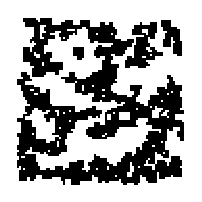
\includegraphics[width=5cm, angle=270]{figures/attractive_20.eps}}
}
\subfigure [Heterophilic (Lacework Pattern)]
{
\label{repulsive_20}
\framebox{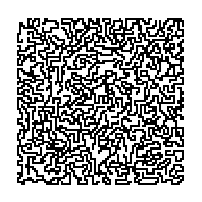
\includegraphics[width=5cm, angle=270]{figures/repulsive_20.eps}}
}
\caption{2D morphologies generated on a $80x80$ lattice using $25$ unit
snakes, at a $50\%$ by volume density. Simulations were run to
quasi-equilibrium. Identical simulation parameters were used for both,
except for the sign of the snake-snake affinity.}
\label{2d_morphology}

\end{figure}

\subsection{Homophilic Blends (Clumping)}
When the snake-snake affinity was greater than the
snake-sea material, clumping into seperate islands of material was observed.
Initial clumping is very fast, producing small islands ($\approx10$ tangled snakes)
that display a collective mobility which produces in the medium term large
islands ($\approx100$ tangled snakes) [Fig. \ref{attractive_20}]. These large islands are fairly
immobile, and further aggregation is archieved by a periodic ejection of
small numbers of snakes ($\approx1-4$ snakes) which are then free to
wander around the lattice, until becoming associated with another island.
This, extremely slow, aggregation eventually produces a full phase
seperation of the material, wherein the small islands eventually
`evaporate', forming one large tangle of snakes.

We believe that experimental samples exist somewhere in the middle-part of
the above process, where a quasi-equilibrium exists. Complete aggregation
and phase separation takes several more decades of time than archieving the
local-clumping.

At lower temperatures, this clumping occures on a more local scale
producing smaller sized clumps distributed across the lattice. As the temperature
increases, the clumps become larger. Once $k_b T \gg E_{int}$, the clump
size decreases and the morphology tends towards a random distribution of
snakes.

We found that $k_b T \approx E_{int}$ gave rise to the most clumped
material, and approached quasi-equilibrium fastest. Therefore a figure of
$k_b T = E_{int}$ was used to generate the majority of simulated samples, in
order to show maximum diversity between the two morphologies.


\subsection{Heterophilic Blends (Lacework Pattern)}
When the affinity between snake-sea was made greater than that for
snake-snake, it had been anticipated that the snakes would avoid each other
and produce a poorly percolating structure. This was indeed demonstrated to
be true for low densities ($<15\%$ in 3D), where the `snakes' kept themselves
separated from one another. However, as the density was increased, some
interesting behaviour emerged. Initially, the increase in density meant that
a random assembly of rods would interact - and so the polymer chains adopted a
loose-spiral formation. 

As the density increased further, the chains were forced into a touching
lacework configuration [Fig. \ref{repulsive_20}]. 
This structure provides enormous interfacial area between the two
polymers in the blend, which we note may have implications for the exciton
lifetime before disassociation into Hole-Electron pair \& rates of
recombination.

Again, excessive temperatures produced a random distribution, and at low
temperatures the blends took a long time to settle into a lacework
structure. A figure of $E_{int} = |k_b T|$ was found to produce the minimally
clumped blend in the shortest time.

\section{CTRW Time of Flight}

A Continue Time Random Walk (CTRW) was used to simulate a Time of Flight
experiment using synthesised blends of the two polymers generated above. A
collection of charge carriers (typically 200) were generated randomly in the first $10\%$ of
the vertical extent of the sample (typical dimensions $1000x50x50$). The
hoppers were constricted to move only within one type of polymer in the
blend. Charge movement was by short range hopping of the charge carriers to
unoccupied lattice sites.

In a CTRW, a list is kept of such `hoppers' with their respective time until they
tunnel, and destination. The simulation time is advanced to that of the
first hopper to move, which is then moved to its intended lattice location.
Any movement with or against the field is considered a contribution to the
current, which was collated into geometric time bins. The hopper then has
the next `hop' chosen, and is reinserted into the queue.

When hoppers reached the far end of the lattice, they were considered to
have been picked up by the electrode, and were removed from the simulation.

For each lattice site, the rate of hopping between near neighbours were
calculated by using Marcusformualism, considering a uniform electric
field across the lattice. These rates, along with a
summation of the total hopping rates, were computed for all lattice sites
and cached for later lookup. Energetic site disorder was
not considered, in order to isolate the effects of morphology, and a figure
of $0.5eV$ was used for the $\lambda$ site deformation energy.

$\gamma = \gamma_0 e^{-  \frac{(\delta E)^2}{4\lambda k_b T} - \frac{r}{r_0}}$

Where the simulation was run at a temperature $T=300K$, and with a tunneling
parameter of $r_0=0.15$ lattice sites.

Each hopper was given a certain wait time by:

$\delta t = - ln(\frac{X}{\gamma_{total}})$

Where $X$ is a random number between $0\rightarrow1$, and $\gamma_{total}$ is the
summation of rates for that lattice site.

The destination for the hopper was chosen by selecting randomly from the
collection of possible jumps, weighted by the relative magnitude of the
rate. If the destination site was found to be occupied by a hopper, another
destination was randomly chosen. If the hopper was found to be trapped by
surrounding hoppers, a `phantom' hop was inserted into the queue, whereby
the hopper `moved' to its on location at a future time, allowing hoppers to
`sleep' until a time by which the surrounding hoppers would have moved away.

\section{Time of Flight Results}

Testing was done with a pure $100\%$ sample, which displayed the expected
charge-sheet like behaviour and postive field-dependence of mobility.
Simulations were then made with the prepared $1000x50x50$ blends of
homophilic \& heterophilic polymer chains at a variety of densities. The
electric field bias was varied from $0.01$ to $0.1$ eV/site, which along
with the $1000$ unit thick lattice, was intended to simulate a $1000nm$
thick blend of conjugated polymer with biases of $10$ to $100$V.

The Heterophilic morpohology was found to produce non-dispersive
`charge-sheet' ToF transients, which became more dispersive as the bias was
increased. This was understood by the existence of `fish-trap' structures
within the morphology. High density morpohologies were found to be
increasingly resistive to this deformation into dispersive transport.
Densities above $17\%$ were found to produce conducting films.

Homophilic morphologies only produced viable ToFs for densities of above
$22\%$. Low ($<35\%$) density morphologies gave rise to entire dispersive
transport at the range of biases sampled, but higher densities exhibited
similar though less pronounced field-responsive dispersive transport.





\begin{figure}[htb]
\centering
\subfigure [Homophilic (Clumping)]
{
\label{attractive_tof}
\framebox{\includegraphics[width=5cm,angle=270]{figures/a_0.25.bin_lattice.dat.ToF_trans.eps}}
}
\subfigure [Heterophilic (Lacework Pattern)]
{
\label{repulsive_tof}
\framebox{\includegraphics[width=5cm,angle=270]{figures/r_0.25.bin_lattice.dat.ToF_trans.eps}}
}
\caption{Simulated Time of Flights generated from $25\%$ density homophilic
\& heterophilic polymer blends. Current versus Time is presented on a
logscale, with the data collated into $150$ geometric timebins. Three biases
are displayed, $0.01, 0.05 \& 0.1 eV/site$. 
}
\label{tofs}
\end{figure}

\section{Conclusions}

\end{document}
